% template for papers with a title page
% see dgstpp.sty for title page info
% format: latex
% last changed: 1 Apr 2015

\documentclass[final]{IEEEtran}

% standard math packages
\usepackage{amsmath,amsfonts,amssymb}
\usepackage{scrextend}
\usepackage{tikz}
\usepackage{hyperref}
\usetikzlibrary{arrows, shapes, plothandlers}
\usepackage{tikz}
\usepackage{tikzscale}
\usepackage{ragged2e}
\usepackage{hyperref}


\usepackage{listings}
\usepackage{color}

\definecolor{dkgreen}{rgb}{0,0.6,0}
\definecolor{gray}{rgb}{0.5,0.5,0.5}
\definecolor{mauve}{rgb}{0.58,0,0.82}

\lstset{frame=tb,
  language=bash,
  aboveskip=3mm,
  belowskip=3mm,
  showstringspaces=false,
  columns=flexible,
  basicstyle={\small\ttfamily},
  numbers=none,
  numberstyle=\tiny\color{gray},
  keywordstyle=\color{blue},
  commentstyle=\color{dkgreen},
  stringstyle=\color{mauve},
  breakatwhitespace=true,
  tabsize=3,
  breaklines=true,
  postbreak=\mbox{\textcolor{red}{$\hookrightarrow$}\space}
}


% Phil Parker's DGS packages, some modified
\usepackage{remexpp,pprroof,dgstpp}

% other packages
\usepackage{setspace}
%\usepackage{hyperref,color}

% "fancy" font
\usepackage{fourier}
\usepackage[T1]{fontenc}
   
% make reference header the right font size
\renewcommand\refname{\Large References}
   
% theorems, remarks, etc using Phil Parker's "remexpp.sty"
\newtheorem{theorem}{Theorem}[section]
\newtheorem{prop}[theorem]{Proposition}
\newtheorem{lemma}[theorem]{Lemma}
\newtheorem{claim}[theorem]{Claim}
\newtheorem{corollary}[theorem]{Corollary}
\newremark{definition}[theorem]{Definition}
\newremark{example}[theorem]{Example}
\newremark{remark}[theorem]{Remark} 

% make rsfs, TeX \cal, and Euler script *all* available
\usepackage{mathrsfs}
\let\rscr=\mathscr
\let\mathscr=\relax
\let\mcal=\mathcal
\usepackage{eucal}
\let\escr=\mathcal
\let\mathcal=\relax

% commutative diagrams with XY-pic
\usepackage[all]{xy}
\SelectTips{cm}{}

\arraycolsep .2em
   
% new commands
\renewcommand{\a}{\alpha}
\newcommand{\Aut}[1]{\textrm{Aut}(#1)}
\newcommand{\B}{\rscr{B}}
\newcommand{\br}[2]{\left[#1,#2\right]}
\newcommand{\bre}{\br{\ }{\,}}
\newcommand{\ddg}{\ddot{\g}}
\newcommand{\dg}{\dot{\g}}
\newcommand{\DGS}{D{\kern-.375em}G{\kern-.2em}S}
\newcommand{\ds}{\oplus}
\newcommand{\eB}{\escr{B}}
\newcommand{\eH}{\escr{H}}
\newcommand{\eI}{\escr{I}}
\newcommand{\eV}{\escr{V}}
\newcommand{\g}{\gamma}
\newcommand{\G}{\Gamma}
\newcommand{\h}{\lal{h}}
\renewcommand{\H}{\rscr{H}}
\newcommand{\hp}{\h_{2p + 1}}
\newcommand{\iso}{\cong}
\newcommand{\lag}{\mathfrak{g}}
\newcommand{\lal}[1]{\mathfrak{#1}}
\newcommand{\n}{\lal{n}}
\newcommand{\pplus}{+\mspace{-10 mu}+}
\newcommand{\R}{\mathbb{R}}
\newcommand{\rS}{\rscr{S}}
\renewcommand{\span}[1]{[\mspace{-3.25 mu}[ #1 ]\mspace{-3.25 mu}]}
\newcommand{\surj}{\rightarrow\kern-.82em\rightarrow}
\newcommand{\tQ}{\widetilde{Q}}
\renewcommand{\v}{\lal{v}}
\newcommand{\V}{\rscr{V}}
\newcommand{\z}{\lal{z}}
%%Alex's defined commands%%
\newcommand{\adx}{ad$_x$ }
\newcommand{\ady}{ad$_y$ }
\newcommand{\adz}{ad$_z$ }
\newcommand{\fj}{\mathfrak{j}}
\newcommand{\fg}{\mathfrak{g}}
\newcommand{\fz}{\mathfrak{z}}
\newcommand{\fv}{\mathfrak{v}}
\newcommand{\fh}{\mathfrak{h}}
\newcommand{\QQ}{\mathbb{Q}}
\newcommand{\ZZ}{\mathbb{Z}}
\newcommand{\RR}{\mathbb{R}}
\newcommand{\CC}{\mathbb{C}}
\newcommand{\NN}{\mathbb{N}}
\newcommand{\FF}{\mathbb{F}}

\makeatletter
\newcommand{\ad}[1]{\mathop{\operator@font ad}\nolimits_{#1}}
\makeatother

% show labels in margin (must be last package added)
\usepackage{showlabels}

% input information for the title page here:
\preprint{}
\title{Apache Apex \\ \normalsize Development Docker Image}
\author{Alexander Jansing}
\address{
   Computer Science Department\\
   State University of New York,\\
   Polytechnic Institute\\
   Utica, NY 13502\\
   USA\\
   \textsf{jansina@sunyit.edu}
}
\date{\today}
\abstract{
Apache Apex is Hadoop YARN-native framework for building distributed applications and applies native streaming to the data processing pipeline \cite{WEISE}. The Apex project was mainly been driven by the company DataTorrent. DataTorrent shut its doors back in May of 2018\cite{WIKI}\cite{DATANAMI}.

This project is designed to help other developers write their own Apache Apex applications by providing an Docker image with Apex, JDK8, and Maven installed. The start-up script provided can be easily changed so that others can pass their project directory as a volume to a container and rapid testing can be performed.
}
\msc{}{}

\begin{document}
\maketitle



%   the main focus of the project (the topic)
\section{Introduction}
\subsection{Apache Apex and Mahlar}
Apache Apex is Hadoop YARN-native framework for building distributed applications and applies native streaming to the data processing pipeline \cite{WEISE}. The Apex project was mainly been driven by the company DataTorrent. DataTorrent shut its doors back in May of 2018\cite{WIKI}\cite{DATANAMI}. The last release of Apex was put out on April $27^{th}$ of the same year; which wasn't that long ago as of the writing of this paper, but looking at the related github repositories and Apache Jira board doesn't do much to inspire confidence in future releases.

Apex comes with Malhar, a codec library of operators used to enable users to speed up their work and in a variety of languages (Java, JavaScript, Python, R, Ruby). Malhar operations are based off of templates and can be easily extended to perform the actions you need. Additionally, Malhar allows the developer to change the properties of an operator at runtime, so the application doesn't need to be brought offline\cite{MALHAR-DOCS}.

This project is designed to help other developers write their own Apache Apex applications by providing an Docker image with Apex, JDK8, and Maven installed. The start-up script provided can be easily changed so that others can pass their project directory as a volume to a container and rapid testing can be performed (see \ref{sec:apex-maven}).

% Your paper must be structured properly (with numbered titled sections), detailing
\subsection{Structure of the Paper}
The summary of the work performed this semester will be laid out as follows:
\begin{enumerate}
  \item the research involved in working with Apache Apex and its potential use case,
  \item how Apache Apex was used; including
  \begin{enumerate}
    \item what was done,
    \item and the challenges faced.
  \end{enumerate}
  \item and finally a reflection on what was and was not accomplished.
\end{enumerate}


%   the relevance of the topic to big data (whether or not your topic is directly related to Spark,
%  and Hadoop)
% \item the research involved in working with Apache Apex and its potential use case,
\section{Research}
\subsection{Process}
Whenever researching a piece of technology to use, especially when software under Apache Software Foundation (\emph{ASF}), plenty of documentation is available on the project's site. Usually, there is enough information there to get started in understanding how and why to use a particular product. Usually one should look beyond the product's page when the software isn't under the ASF; as many companies are looking to inflate their egos or sell a license.

In the case of this project, I used the Apache Apex project page \cite{APEX}, the provided ReadTheDocs pages\cite{APEXrtd_dt} \cite{APEXrtd_apache} \cite{MALHAR-DOCS}, a presentation from a DataTorrent employee, Thomas Weise \cite{WEISE}, Wikipedia and its references \cite{WIKI} \cite{DATANAMI} to help me understanding how the framework was designed to work. Since Apex is covered under the ASF and its primary driving company, DataTorrent, went under in May 2018, I wasn't too concerned with being convinced to buy a license.

\subsection{Use Case}
As was stated in the introduction, Apache Apex is Hadoop YARN-native framework for building distributed applications and applies native streaming to the data processing pipeline \cite{WEISE}. YARN-native means that applications developed using the Apache Apex API can be deployed directly onto an HDFS clustering using YARN without installing any new software \cite{WEISE2}.

Apache Apex can be thought of as an alternative to Apache Spark for performing analytics. It appears that Apex was inspired, at least partially, by Spark as seen by its use of a \emph{DAGs} (Directed acyclic graphs) pattern of arranging code (see \ref{sec:overview}).

Another of Apache Apex's lesser known features is that it supports automatic scaling with the demands placed upon itself \cite{WEISE2}. The ability to automatically scale an application up or down based on the current needs of a system is a great feature for any framework or application to have and it a major selling point for some other software out there, i.e. Cloud Foundry \cite{CF}.

Apache Apex's primary use case seems to take advantage of an existing HDFS cluster, using YARN (Mesos support was never released \cite{APEX-JIRA}), to perform streaming analytics; i.e. training LSTMs (Long short-term memory neural networks) or reading data that continually streams in from a source.

\section{Using Apex}
\subsection{Quick Overview of the Apache Apex API} \label{sec:overview}
The Apache Apex API consists of two primary units; \emph{Operators} and DAG. Operators are the most basic units of Apex applications and the vertices of the DAG. The DAG object the graph representation of the Apex application and describes how data streams in and out of Operators (\autoref{fig:apex-app})\cite{APEX-DOCS}.

\begin{figure}
  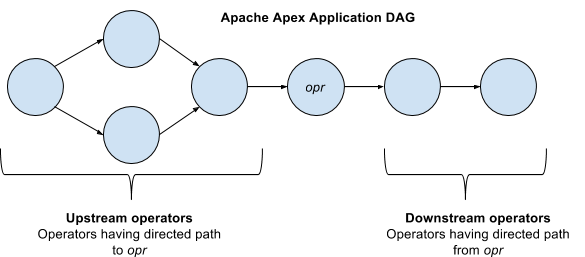
\includegraphics[scale=.4]{../images/apex-dag}
  \caption{Apex Application DAG and Operators}\cite{APEX-DOCS}
  \label{fig:apex-app}
  \centering
\end{figure}

%   the work you have actually done for the project (code, etc.)
%     \item what was done,
\subsection{Work Accomplished}
%   the challenges in using the software relevant to your topic (installation, etc.)
%     \item and the challenges faced.
During my survey of Apache Apex, I worked my way through some of the examples in the apex-malhar (see \ref{sec:repos}), primarily the WordCount example. Using the WordCount example as a starting point, I wrote my own Operators (WordCountInput and MapReducerFileOutputOperator (\ref{sec:map-reduce})) and added them to my application's DAG.

In addition of the basic word counting application, I expanded on the apex-sandbox (\ref{sec:apex-downloads}) to create apex-maven (\ref{sec:apex-maven}). The apex-maven image is a developer Docker image that eliminates the intermediate need to build your project locally, then go into the apex-sandbox to run your project. Instead, the developer can now build Apex projects from within an apex-maven container and launch it within the same terminal window.

The apex-maven image uses apex-sandbox as a starting point and further includes JDK8, Maven, and the apex-malhar git repository, built; meaning that the Malhar library code is included in the image's \textsl{\textasciitilde/.m2/repository/}.

\section{Conclusion}
\subsection{Challenges}
Working with a new framework is always challenging. It gets easier the more frameworks you've been exposed to, but there is always a learning curve. Apache Apex follows this pattern. An overview of how Apex's applications was briefly explained in \ref{sec:overview}. More could have been learned in the pursuit of this project, but Apex's framework was much easier to understanding since I am familiar with reading the documentation associated with Apache Foundation project and Apex shares some of its DAG pattern with Spark.

%   your self-evaluation (what you managed to accomplish and what you failed to complete)
%   \item and finally a reflection on what was and was not accomplished.
\subsection{Reflection}
For this project, I had originally intended to perform a series of work count analytics and later translate those into byte-array counts; via the shingling of the bytes as they streamed into the source Operation vertex. Then, I wanted to find combinations of bytes that did not occur within a given file and replace the shingles to compress the file; providing the series of replacements after the EOF of the original file as a way to reverse the compression.

This project idea was a bit too ambitious to complete given that I needed to learn a whole new framework in the processing and the time provided. While running through the WordCount examples and trying to write my own Operators inspired by others I found (credited in code), I realized I wasn't going to be able to finish the project in time. With that in mind, I decided to get the word-count MapReduce DAG in working order and expand on the apex-sandbox Docker image provided by the Apache Apex project (\ref{sec:repos}) to create an image that developers could use to speed up testing of Apex applications.

\newpage
\section{Appendix}

\subsection{Code snippets and links}
  \subsubsection{MapReduce}\label{sec:map-reduce}
  \url{https://github.com/apjansing/apex-maven/tree/master/src/MapReduce}

  \subsubsection{apex-maven}\label{sec:apex-maven}
  \begin{enumerate}
    \item[$\cdot$] \url{https://github.com/apjansing/apex-maven/blob/master/src/docker/Dockerfile}
    \item[$\cdot$] \url{https://hub.docker.com/r/apjansing/apex-maven/}
  \end{enumerate}
  
  \subsubsection{pull\_and\_start\_dev\_apex\_docker.sh}\label{sec:start-script}
  \begin{lstlisting}
    #!/bin/bash
    JANSING_PROJECT_HOME=`(git rev-parse --show-toplevel)`
    JANSING_REPO_NAME=`(basename $JANSING_PROJECT_HOME)`
    
    docker pull apjansing/apex-maven
    docker run -it --name=apex -v $JANSING_PROJECT_HOME:/home/ apex/$JANSING_REPO_NAME -p 50070:50070 -p 8089:8088 apex-maven
  \end{lstlisting}
  
\subsubsection{MapReduce Output}\label{sec:map-reduce-output}
  \begin{lstlisting}
    {monstrous=1, allah=1, xlv=1, xxxvii=1, bag=1, dutch=1, xxiv=1, vii=3,...},
    {... cheerless=1, monstrous=4, flinty=1, been=12, gaping=1, ...},
    {... ticking=1, monstrous=1, been=64, mostly=2, ...},
    {... account=5, monstrous=6, been=60, unquestion=1, ...}
  \end{lstlisting}


%   the references you have used (books, papers, web sites, etc.); remember that you must
%  give proper credits (i.e. proper references) to work you use that is not your own.
\subsection{Source locations}

\subsubsection{Apex Documentations}\label{sec:apex-docs}
\begin{enumerate}
  \item[$\cdot$] \url{http://apex.apache.org/docs/apex}
  \item[$\cdot$] \url{http://apex.apache.org/docs/malhar}
  \item[$\cdot$] \url{http://apex.apache.org/docs/apex/apex_development_setup/#creating-new-apex-$\cdot$project}
\end{enumerate}

\subsubsection{Github Repositories}\label{sec:repos}
\begin{enumerate}
  \item[$\cdot$] \url{https://github.com/apjansing/apex-maven}
	\item[$\cdot$] \url{https://github.com/apache/apex-core}
	\item[$\cdot$] \url{https://github.com/apache/apex-malhar}
	\item[$\cdot$] \url{https://github.com/apache/apex-site}
\end{enumerate} 

\subsubsection{Apache Apex Downloads}\label{sec:apex-downloads}
\begin{enumerate}
	\item[$\cdot$] \url{http://apex.apache.org/downloads.html}
	\item[$\cdot$] \url{https://hub.docker.com/r/apacheapex/sandbox/}
\end{enumerate}

\begin{thebibliography}{99}
  \bibitem{APEX}
  Foundation, A. (2018). Apache Apex. [online] Apex.apache.org. Available at: \url{https://apex.apache.org/} [Accessed 5 Nov. 2018].
  
  \bibitem{WIKI}
  En.wikipedia.org. (2018). Apache Apex. [online] Available at: \url{https://en.wikipedia.org/wiki/Apache_Apex [Accessed 10 Nov. 2018]}.
  
  \bibitem{WEISE}
  Weise, T. (2016). Architectual Comparison of Apache Apex and Spark Streaming. [online] Available at: \url{https://www.slideshare.net/ApacheApex/architectual-comparison-of-apache-apex-and-spark-streaming} [Accessed 10 Nov. 2018].

  \bibitem{APEXrtd_dt}
  Dt-docs.readthedocs.io. (2018). Beginner's Guide - DataTorrent Documentation. [online] \url{Available at: https://dt-docs.readthedocs.io/en/latest/beginner/} [Accessed 10 Nov. 2018].

  \bibitem{APEX-DOCS}
  Apex.apache.org. (2018). Apache Apex Documentation. [online] Available at: \url{http://apex.apache.org/docs/apex/} [Accessed 10 Nov. 2018].

  \bibitem{MALHAR-DOCS}
  Apex.apache.org. (2018). Apache Apex Malhar Documentation. [online] Available at: \url{http://apex.apache.org/docs/malhar} [Accessed 10 Nov. 2018].

  \bibitem{DATANAMI}
  Leopold, G. (2018). DataTorrent, Stream Processing Startup, Folds. [online] Datanami. Available at: \url{https://www.datanami.com/2018/05/08/datatorrent-stream-processing-startup-folds/} [Accessed 10 Nov. 2018].

  \bibitem{WEISE2}
  Weise, T. (2018). Stream Processing use cases and applications with Apache Apex | Big Data Spain. [online] Bigdataspain.org. Available at: \url{https://www.bigdataspain.org/2016/program/fri-stream-processing-use-cases-applications-with-apache-apex.html} [Accessed 12 Dec. 2018].

  \bibitem{CF}
  Yang, B. (2018). cloudfoundry-incubator/app-autoscaler. [online] GitHub. Available at: \url{https://github.com/cloudfoundry-incubator/app-autoscaler\#deploy-and-offer-auto-scaler-as-a-service} [Accessed 12 Dec. 2018].

  \bibitem{APEX-JIRA}
  Issues.apache.org. (2018). Apache Apex Core - ASF JIRA. [online] Available at: https://issues.apache.org/jira/projects/APEXCORE/summary [Accessed 12 Dec. 2018].
\end{thebibliography}
\end{document}